\documentclass[12pt, letterpaper]{article}
%\documentclass[ letterpaper]{article}

\usepackage{amsmath}
\usepackage{graphicx}

\setlength{\textheight}{9.25in}
\setlength{\textwidth}{6.5in}
\setlength{\evensidemargin}{-.25in}
\setlength{\oddsidemargin}{-.25in}
\setlength{\topmargin}{-.75in}
\setkeys{Gin}{width=0.5\textwidth}
 
\newcommand{\code}{\texttt}
\newcommand{\degree}{\ensuremath{^\circ}}
\newcommand{\blank}{\texttt{\_\_\_\_\_\_\_\_\_\_\_\_\_\_\_\_\_\_\_\_\_\_\_\_\_\_\_}}
\usepackage{Sweave}
\begin{document}

\begin{center}\textbf{\Large Body Mass Scaling Example} \end{center}
%\begin{center} \today \end{center}
\bigskip


Marsupial mammals scale in BMR (basal metabolic rate) with mass (in g) according to the following equation (see Withers 1992 Table 4-5):

\begin{align*}
BMR &= a * Mass^b \\
	&= 47.6M^{0.75} J/hr 
\end{align*}	


\section*{Questions:}
\begin{enumerate}
\item Who has higher BMR? A 10g or 10Kg animal?  \\ \\
\item Who has the higher mass-specific BMR?  \\ \\ \\ \\
\item Plot lines for mass vs. BMR and mass vs. mass-specific BMR on a log-log plot, indicate where the 10g and 10Kg animal lie on each. (First Log$_{10}$-transform the equations -- it's easier to plot). \\ 
\end{enumerate}

\begin{right}
  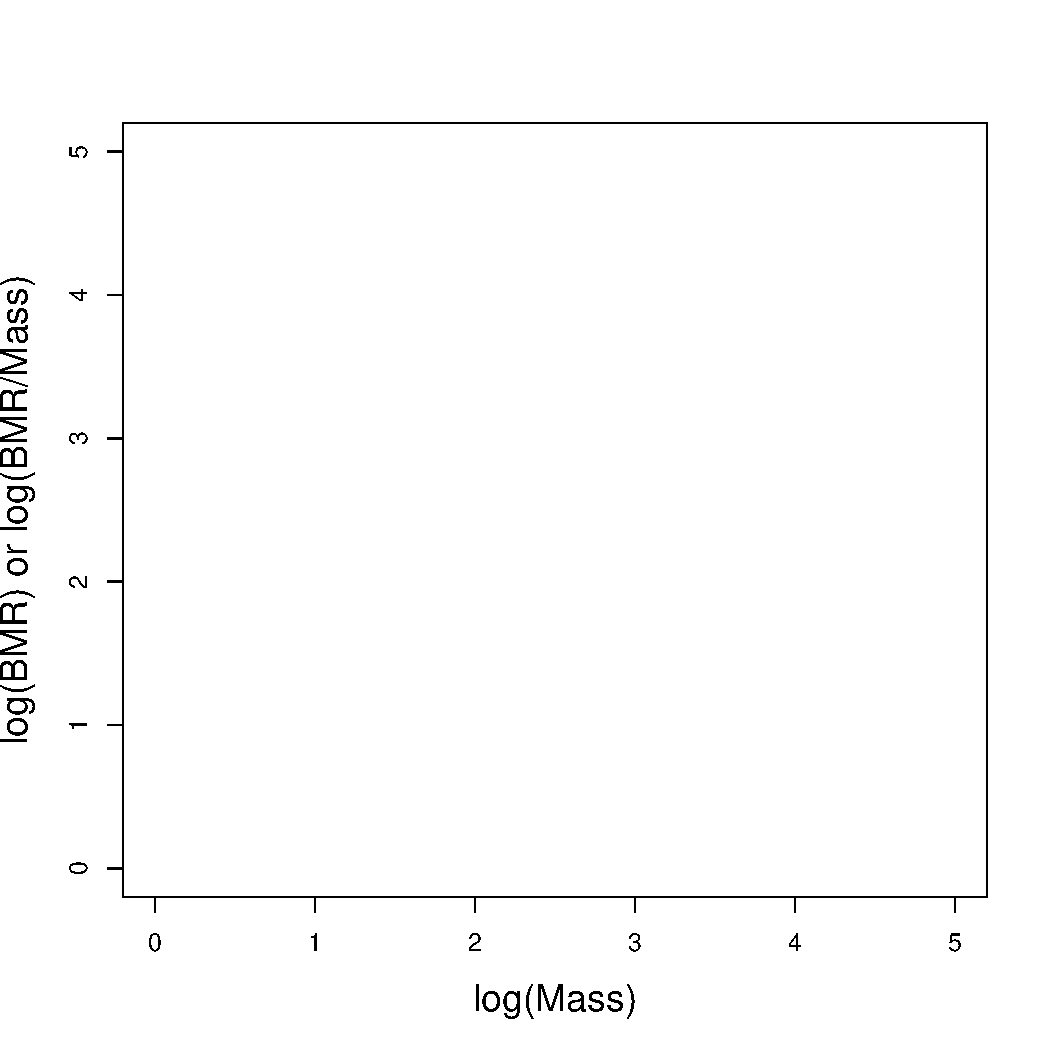
\includegraphics[width=100mm]{blankplot}
\end{right}
\end{document}
